\documentclass[11pt]{article}

\usepackage{amsmath}
\usepackage{amsthm}
\usepackage{booktabs}
\usepackage{dcolumn} 
\usepackage{epstopdf}
\usepackage{fourier}
\usepackage{fullpage}
\usepackage{graphicx}
\usepackage{hyperref}
\usepackage{longtable} 
\usepackage{natbib}
\usepackage{rotating}
\usepackage{tabularx}
\usepackage{tikz} 
\usepackage{xcolor} 
\usepackage{setspace}

\hypersetup{
  colorlinks = TRUE,
  citecolor=blue,
  linkcolor=red,
  urlcolor=black
}

\DeclareMathOperator*{\argmax}{\arg\!\max}

\newcommand{\starlanguage}{Significance indicators: $p \le 0.05:*$, $p \le 0.01:**$ and $p \le .001:***$.}  

\newif\ifdraft

%\drafttrue % or 
\draftfalse

\ifdraft
\newcommand{\important}[1]{\textcolor{red}{\textbf{#1}}}
\usepackage{setspace}
%\doublespacing
\else
\newcommand{\important}[1]{#1}
\fi

\begin{document} 

\title{Peer-to-Peer Rental Markets:\\
Some Thoughts on the ``Sharing Economy''}

\date{\today}

\author{John J. Horton \\ Leonard N. Stern School of Business \\ New
  York University\footnote{Author contact information, datasets and
    code are currently or will be available at
    \href{http://www.john-joseph-horton.com/}{http://www.john-joseph-horton.com/
    Thanks to Andrey Fradkin, Ramesh Johari, Arun Sundararajan, Samuel Fraiberger, Hal Varian and Joe Golden for helpful discussions and comments.}}
  \and 
  Richard J. Zeckhauser \\ Harvard Kennedy School \\ Harvard University
}
\maketitle

% grep '\\important{' sharing.tex | sed 's/\\important{//g' | sed 's/}//g'
% Sarah Cannon ; Lawrence Summers
% http://blogs.hbr.org/2014/10/how-uber-and-the-sharing-economy-can-win-over-regulators/
% http://blogs.hbr.org/2013/01/from-zipcar-to-the-sharing-eco/

\begin{abstract} 
Recent technological advances and entrepreneurial efforts have created a number of new peer-to-peer rental markets in which owners can rent out their durable goods. 
We consider the emergence of such a market and determine the market clearing rental rate, the patterns of trade and the surplus unlocked for different types of consumers. 
Our analysis considers both a short-run, before consumers can revise their ownership decisions and a long-run, in which they can. 
A survey of consumers finds broad support for the modeling conventions
used---namely that ownership is determined by a forward-looking evaluation of planned usage.
We also explore the factors that are permitting these new markets to flourish. 
\newline \newline 
\noindent JEL J01, J24, J3 
\end{abstract} 

\onehalfspacing

% TODO: Better title?
% TODO: Cite to that Slee guy; Dean Baker and the platform cooperative guy for criticisms
% TODO: What are the best insights from the theory model? Emphasize them in the introduction
% TODO: Add citations to the ``factors'' section of the paper
% TODO: Pass through in the BMC short-run - can we say anything about incidence? 
% D[2\left[ (1-\theta)\alpha_L - (1-\alpha_H) \theta \right], \theta] = 2 [1 - (alpha_H - \alpha_L)] + \gamma

\section{Introduction}
In traditional rental markets, owners hold assets to rent them out.
In recent years, a new kind of rental market has emerged, with the markets created by technology startups firms 
In these ``sharing economy'' markets, owners sometimes use their assets for personal consumption, and sometimes rent them out.
To be sure, some renting by consumer-owners has long existed, but it was largely confined to expensive, infrequently used goods, such as vacation homes and pleasure boats.
More often, consumer-owner goods were shared among family and friends, without explicit payment.
In contrast, these P2P rental markets are open markets and the good is ``shared'' for payment. 

Perhaps the most prominent example of a P2P rental market is Airbnb, which allows individuals to rent out spare bedrooms, apartments or even entire homes. 
Airbnb and platforms like it have been heralded by many, as they they promise to expand access to goods, diversify individual consumption, bolster efficiency by increasing asset utilization and provide income to owners \citep{sundararajan2013zipcar}.
The business interest in these platforms has been intense; Airbnb alone has attracted nearly \$800 million in venture capital investment\footnote{\href{http://www.crunchbase.com/organization/airbnb}{http://www.crunchbase.com/organization/airbnb}}
These companies have also attracted policy interest, much of it negative. 
Critics charge that the primary competitive advantage of these platforms is their ability to duck costly regulations---regulations that often are intended to keep costs from being imposed on third-parties.\footnote{
  See \cite{horton2014tragedy} for a discussion of the externalities imposed by Airbnb-style subletting in rented apartments.
}   
A better understanding of these markets, and progress in resolving this policy debate requires an elucidation of what economic problem these markets address, why they are emerging and what their properties are likely to be in both the short- and long-runs. 
Providing this elucidation is the goal this paper. 

Our first major question is why P2P rental markets are flourishing now.
The economic problem P2P rental markets are attempting to solve---under-utilization of durable goods---is hardly new.  
We argue that although technological advances, such as the mass adoption of smart-phones and the falling cost of developing and running large web sites, while clearly important, only provide part of the story. 
P2P rental markets rely heavily on the hard-won industry experience in the design and management of online marketplaces.
In particular, recommender systems and reputation systems, which emerged during the early days of electronic commerce, are relied on extensively in P2P rental markets.  
This knowledge allows P2P rental platforms to overcome---or at least substantially ameliorate---market problems such as moral hazard and adverse selection.  
We develop this argument in more depth and point out relevant works from the literature. 

Our second major question is what are the economic properties of P2P rental markets. 
For example, what determines the rental rate and the quantity exchanged in a P2P rental market? 
How much total surplus is ``unlocked'' by the P2P rental market and how is it distributed? 
How does the short-run rental rate---where existing owners rent to non-owners---differ from the long-run in which owners and non-owners alike can revise their ownership decision in light of the existence of a P2P rental market?
Does overall ownership increase or decrease and who owns in the new equilibrium?
When there are substantial bringing-to-market costs (such as labor, depreciation and transaction costs), who bears them and how does it affect the short- and long-run equilibria? 

% Model description
To address these questions, we develop a simple model in which consumers initialy decide whether to purchase a good based on their expected usage.
We consider a case where there are owners and non-owners, with the owners using the good less than 100\% of the time and non-owners, while not purchasing the good, would use it some of the time if they owned the good. 
These owners and non-owners then trade with each other after some technological/entrepreneurial shock that creates a P2P rental market.
The owners rent their unused capacity to non-owners, plus however much of the good becomes available because economize on their own usage to make more the good available for the rental market.

While we assume a purchase price that splits consumers into owners and non-owners, other equilibria are possible, such as one where everyone owns the good.
For a given set of consumer valuations, there is a range of product market prices that can support a short-run P2P rental market.
The price has to be low enough that the high-types own (i.e., there is a product market in the good) in order to provide the supply, but not so low that everyone simply owns the good, in which case there is no demand.\footnote{
  Of course, in the long-run ownership decisions can be revised.
}   

After the P2P rental market emerges, owners and non-owners use the good as if they were renting the good at the market-clearing rental rate. 
Renters do face the rental rate, while for owners, the possibility of rental creates a new opportunity cost for their own usage. 
The rental rate is increasing in the valuation of the owners, which reduces supply, and the valuation of the renters, which increases demand. 
The short-run rental market does not necessarily clear: if pre-P2P rental excess capacity exceeds demand, there is a glut. 
In practice, the inherent transaction cost of bringing excess capacity to the market provides a price floor.     

In addition to the short-run, we consider a long-run where owners and renters alike can revise their ownership decisions. 
If the short-run cost to rent the good 100\% of the time is below the purchase price, then ownership is less attractive, which will reduce \emph{purchase} demand for product, and vice versa. 
In the long-run P2P rental market equilibrium in the absence of bringing-to-market costs, the purchase price equals the rental rate and owners and renters receive the same utility, decoupling individual preferences from ownership. 
The model offers an intuitive test for whether total ownership will decrease in the long-run:
ownership decreases if the short-run rental rate is below the purchase price. 

Surplus increases in both the short and long-run P2P rental market equilibria.
Although owners have less consumption, they are compensated with rental income that exceeds the utility loss. 
The greatest gains in surplus are obtained when original non-owners value the good nearly as much as owners, suggesting that good where income explains ownership could offer the greatest increase in surplus. 
The existence of a P2P rental market allows for a higher maximum price in the product market, as it can generate positive demand for a good at prices for which even high-types would not buy without the possibility of rental. 

We also consider bringing-to-market costs.
These costs change the model outcomes is several important ways.
First, if these costs are sufficiently high, no P2P rental market can exist.
If the market can exist, the bringing-to-market costs raise the rental rate and lower the quantity of the good transacted in the market.
However, bringing-to-market costs are not fully passed through in the rental rate.
The presence of bringing-to-market costs changes the predictions about long-run ownership, in that consumers with a higher valuation of the good have a preference for owning.
As in the short-run case, in the long-run there is incomplete pass through of the bringing-to-market costs, which implies that no party without consumption value from owning the good would find it profitable to compete in the rental market (though this result depends on there being no scale economy in renting). 

In the model, we consider the possibility that different goods might differ in the cost required to bring them to market and how this affects the P2P rental market. 
Some of these bringing-to-market costs are straightforward, such as labor, depreciation and complementary consumables.
For example, driving with Uber requires your labor, puts additional miles on your car and consumes gas.
However, another aspect that is relevant to bringing-to-market costs is how amenable a good is to ``temporal division'' and hence renting.
For example, goods where usage can be planned for and easily adjusted are easier to rent out with little lost utility to the owner. 
Similarly, goods that are used in large chunks of time---with no use in between---are more amenable to rental than goods that have usage broken up into many small chunks of time.

Our final question is how the usage patterns for different goods is likely to affect bringing-to-market costs.
To do this, a convenience sample of consumers were asked a series of questions about a good (e.g., a BBQ grill) such as whether they own one, whether they have lent it out or borrowed it and, how much they do or would use it (depending on ownership). 
If they do not own it, they were asked why. 
We also asked questions about how the good in question is characteristically used, focusing on how predictable that usage is and the typical size of usage ``chunks.'' . 
Finally, the respondent was asked for their household income.  
We selected a number of goods and encouraged respondents to answer our questions about multiple goods, as this allows us in some cases to control for the identity of the respondent. 

Our main findings are that for only a small number of goods (e.g., vacation homes) is income important in determining ownership. 
For other goods, planned usage was the primary driver, supporting our basic modeling framework.  
Looking across the population, goods that are owned more frequently are rented less frequently, with the notable exception of cars.
There is also a strong correlation between goods have predictable usage (``you know when you are going to use it'') and the good being used in large chunks of time.
This is useful for a P2P rental market, as it means a larger class of goods is likely to have lower bringing-to-market costs.  

We conclude with some thoughts on how P2P rental markets might evolve.
Our analysis focuses on a single homogeneous good, but a key advantage of P2P rental markets might be in facilitating greater diversity in goods offered and consumed. 
In addition to whatever direct utility this diversification provides, it might also increase the stock of people with direct experience with a particular good, which combined with the continued proliferation of consumer-generated reviews and ratings might stimulate quality improvements. 
In that same vein, we also discuss how the producers of goods might do more than simply improve quality, but also explictly modify the goods to make them more or less amenable to rental, depending on their own market power. 
 
\section{Factors explaining the rise of peer-to-peer rental markets}

The somewhat obvious economic rationale for P2P rental markets is that the owners of most durable goods use them far less than 100\% of the time.
The excess capacity that this under-utilization generates could be rented out.
The demand side in such a market would be non-owners who would like to use the good, but not enough to purchase it.\footnote{
A non-owner might mean a non-owner in a particular place and time. 
Many Airbnb guests own homes---they just don't own homes everywhere. 
} 
Given the obvious rationale for these markets, why have they only begun to flourish in recent years? 

It is useful to consider what problems the creator of a potential rental market would have to overcome.
As with any market, there are the typical search costs, such as finding and evaluating trading partners and the Internet certainly dramatically reduces these costs \citep{bakos1997reducing}.
Furthermore, there is now nearly 20 years of industrial experience in building online marketplaces and solving their characteristic problems. 
However, informational problems are but one obstacle in creating rental markets; the other is resources. 

Individuals lack the resources of firms that have historically dominated rental markets. 
For example, individuals lack marketing budgets and expertise, ways of accepting payments that are convenient for customers, standard contracts and procedures to draw upon, well-adapted insurance products, procedures and facilities for re-setting goods after use, and so on.\footnote{
  As it is, even ostensibly ``peer'' platforms do seem to tilt towards quasi-firms that can reap economies of scale or enjoy other firm benefits.
  For example, there are Uber drivers that manage fleets of vehicles and Airbnb ``hosts'' with multiple properties. 
  }
For P2P rental markets to draw in individual owners, the platform must fill in these gaps and give them firm-like resources. 
Because of both the lack of firm-like resources and the inherent information problems of rental markets, consumer-owned goods have historically just been shared effectively and often been between family members, neighbors and friends rather than strangers, except when the potential gains from trade are quite large (such as in the example of vacation home and boat rentals). 

P2P rental markets have emerged as entrepreneurs have taken advantage of technological advances to build facilitating platforms. 
The platforms lower transaction costs and provide individual owners tools previously only available to the firm. 
The maturation and increasing penetration of the Internet and the proliferation of smart phones, high resolution cameras and so on---were the technological shock that made these P2P rental markets feasible. 
However, these P2P rental markets have also stood on the shoulders of their electronic commerce predecessors, such as eBay, that made strides towards solving some of the informational problems inherent to online market places. 

Like all software companies, platforms have benefited from the rise of the Internet, which has radically increased the supply of potential users on both sides of the markets. 
They have also benefited from improving industrial knowledge about how to build and maintain large websites.
The cost of creating such sites has plummeted. 

A key challenge in all markets is facilitating trust among strangers, and this problem is more acute in P2P rental markets, given the ``opportunity'' renters have to destroy or misuse the owner's capital.
In most markets, the buyer's type does not matter to the seller; in rental markets, the buyer's type can be critical. 
Facilitating trust is not a solved problem in online markets, but the experiences of early electronic commerce pioneers such as eBay provided P2P rental market entrepreneurs a number of ready-made solutions to market problems related to trust. 
The flaws in early versions of these systems---such as the ability of and inclination of parties to condition their feedback on their trading partner's feedback---also clearly influenced the design of follow-on systems used in P2P rental markets. 
The rise of social networks such as Facebook has given platforms new opportunities to inject information into the the platform that parties can use in their decision of whether to contract. 

Online markets in general lack many of the market-thickening coordination mechanisms available in offline markets such as coordinating on time and geography.\footnote{
  Buyers and sellers of stocks benefit from agreeing that the New York Stock Exchange is open from 9:30-4:00.
  Geography also matters; buyers and sellers of vegetables benefit from agreeing that the Union Square green market is located in the northwest side of the Union Square Park.
}
To compensate for the lack of geography and time as a coordinating mechanism, online marketplaces to create taxonomies and extensive classification of goods.
A complementary approach is to make extensive use of search algorithms and recommendation systems \citep{resnick1997recommender, adomavicius2005toward}.
These kids of approaches are particularly important in P2P rental markets because the goods being rented are often highly differentiated, as are consumer preferences, making matching more important. 

In addition to simply finding each other, would-be trading partners must asses each other and the goods being traded. 
These assessments are aided by verifiable measurements made by the platform on a number of dimensions, including past market history. 
As \cite{varian2010computer} points out, advances in information technology are often advances in measurement.  
Consider that Uber is only possible because both sides of the market now carry with them taximeters (when running the appropriate software) at all times: 
a smart-phone with GPS technology allows for the precise measures of distance traveled.
In fact, this computer-mediated approach works even better than the traditional taximeter in that both parties can verify that the best route was taken. 
The proliferation of high-resolution digital cameras built into smart-phones have similarly made it easier for parties to inspect goods ex ante (Airbnb in particular benefits from this innovation).  
 
Platforms enjoy scale economies for many things that individual owners would find costly. 
For example, they handle credit card payments. 
They create tools for ``self-serve'' marketing (such as through attractive profile pages) and through general platform marketing to bring renters to the platform. 
They also create software tools that let owners manage their availability, learn about the attributes of potential renters and so on. 

% \begin{table} 
% \begin{tabular}{lll}
% Airbnb     & Lodging & \\ 
% RelayRides & Transportation & \\ 
% Boats      &  & \\ 
% Equipment  &  & \\ 
% \end{tabular} 
% \end{table} 

\section{Model} \label{sec:model}

Before anyone can ``share,'' someone has to own and others have to not own.
The first task of our model is explain this division of consumers into owners and non-owners. 
Our model is built from the notion that goods can usefully be thought of as having an intensive margin of usage, which in turn drives the extensive margin decision (i.e., ownership). 
The assumption that consumers must consider the time required to use a good in making their consumption plan is similar in spirit to \cite{becker1965theory}.
The possibility of sharing a good is similar in spirit to \cite{varian2000}.
Varian in particular discusses---in the context of information goods---how planned usage affects the rent-versus-own decision. 

We first consider what happens when the possibility of P2P rental emerges, which allows the existing pool of owners to rent to non-owners. 
First, we assume that there are no bringing-to-market costs (such as labor and transaction costs).
We determine the equilibrium rental rate, the quantity transacted and the change in consumer surplus. 
Next we introduce bringing-to-market costs and see how this changes the short-run equilibrium and whether a P2P rental market can emerge. 

We then turn our attention to the long-run case, where owners and non-owners can revise their ownership decisions.
First we derive the equilibrium without any bringing-to-market costs and derive who owns in equilibrium and what happens to total ownership.
Then we perform the same analysis but assume non-zero bringing-to-market costs. 

\subsection{Consumer decision about ownership based on expected usage}  
Every consumer has a unit of time to allocate to various activities, some of which involve using a good.  
Consumers have to decide how much time, $x \in [0,1]$, to devote to using a particular good. 
There is decreasing marginal utility from use of the good: 
the consumer receives a benefit of $b(x) = 2\alpha x$, but as also incur cost $c(x) = x^2$,  
where $\alpha \in (0,1)$ parametrizes their valuation of the good.
With the functional forms chosen, $\alpha$ has a convenient interpretation, which is that $\alpha$ is the fraction of the time a good would be used by an owner. 
The cost of usage, $c(x)$, as the opportunity cost of time, which grows as more time is spent with the good in question rather than with the next best alternative use of ones' time.

The consumer's utility for a given $x$ is $u(x) = b(x) - c(x) = 2 \alpha x - x^2$, and so individual usage conditional upon owning the good is $x^* = \alpha$ and indirect utility is 
\begin{align}
v(\alpha) = u(x^*) = \alpha^2.  
\end{align} 
The purchase price of the good is $p$ and so a consumer will buy the good only if $\alpha^2 > p$. 
Figure~\ref{fig:consumer} illustrates the consumer's problem, showing the utility from various levels of usage depending on consumers with different values of $\alpha$.
The usage solution for each consumer is their $\alpha$ parameter and since indirect utility is just $\alpha^2$, the optimal usage for each value falls along the curve traced out by $x^2$.
The purchase price $p$ determines who purchases the good, with all those having $\alpha^2 > p$ deciding to own and those below choosing not to purchase the good. 


\pgfmathsetmacro{\alphaOne}{0.40}
\pgfmathsetmacro{\xstarOne}{\alphaOne}%
\pgfmathsetmacro{\ustarOne}{2*\alphaOne * \alphaOne - \alphaOne^2}%

\pgfmathsetmacro{\alphaTwo}{0.55}
\pgfmathsetmacro{\xstarTwo}{\alphaTwo}%
\pgfmathsetmacro{\ustarTwo}{2*\alphaTwo * \alphaTwo - \alphaTwo^2}%

\pgfmathsetmacro{\alphaThree}{0.75}
\pgfmathsetmacro{\xstarThree}{\alphaThree}%
\pgfmathsetmacro{\ustarThree}{2*\alphaThree * \alphaThree - \alphaThree^2}%

\begin{figure}
\caption{Consumer's optimal usage of a good and resultant decision about whether to purchase that good}
\label{fig:consumer} 
\begin{center}
\begin{tikzpicture}[scale=5]
\draw (1,0) node[below]{$x$} -- (0,0) --(0,1) node[left]{$u$};
\draw[thick, domain=0:0.98] plot (\x, {2.0 * \alphaOne *\x - \x*\x});
\node[align=right] at (1, 2.0 * \alphaOne - 1){$\alpha = \alphaOne$};
\draw[dotted] (\xstarOne, 0.0) to (\xstarOne, \ustarOne);

\draw[thick, domain=0:0.95] plot (\x, {2.0 * \alphaTwo *\x - \x*\x});
\node[align=right] at (1, 2.0 * \alphaTwo - 1){$\alpha = \alphaTwo$};
\draw[dotted] (\xstarTwo, 0.0) to (\xstarTwo, \ustarTwo);

\draw[thick, domain=0:0.95] plot (\x, {2.0 * \alphaThree *\x - \x*\x});
\node[align=right] at (1, 2.0 * \alphaThree - 1){$\alpha = \alphaThree$};
\draw[dotted] (\xstarThree, 0.0) to (\xstarThree, \ustarThree);

\draw[thick, dotted, domain=0:0.95] plot (\x, {\x*\x});

\draw[ultra thick] (0, 0.35) to (1, 0.35) node[right]{$p$}; 

\node[align=left] at (1, 1){$u(x^*) = \alpha^2$};

\draw[<->, red, ultra thick] (1.2,0)  -- (1.2, 0.35) ;
\node[red, align = left] at (1.5, 0.17) {Consumer\\does\\not\\buy};

\draw[<->, green, ultra thick] (1.2,0.35)  -- (1.2, 1) ;
\node[green, align = left] at (1.5, 0.65) {Consumer\\buys};
\end{tikzpicture}
\\
\begin{minipage}{0.50 \linewidth}
  \emph{Notes:} This figure illustrates the utility derived from different levels of usage of a good, with individuals differing in their value from usage based on their $\alpha$ parameter. 
\end{minipage}
\end{center}
\end{figure} 


Note that all owners have an amount of time $1 - x^*$ when they are not using the good.
This unused capacity is what they will be able to rent out, plus however much more capacity becomes available when they economize their own usage.

\subsection{Three consumption possibilities with two consumer types but no rentals} 
There are three important potential market configurations with respect to ownership:
(1) everyone owns (2) no one owns and (3) some own and other do not.
For our purposes, the interesting case is (3).
A simple way to obtain this possibility is to assume two consumer types: $\alpha_H$ and $\alpha_L$ with $\alpha_H > \alpha_L$ and to assume a price that divides consumers into owners and non-owners, namely a $p$ such that $\alpha_H^2 > p > \alpha_L^2$.
Assume that there is a unit mass of consumers, with a fraction $\theta$ being high-types with $\alpha = \alpha_H$ and the remaining $(1-\theta)$ consumers being low-types with $\alpha = \alpha_L$. 

The product market demand curve for the good is 
\begin{align} \label{eq:demand}
   D(p) = \left\{
     \begin{array}{ll}
       0 & : p > \alpha_H^2\\
       \theta & : \alpha_H^2 \ge p > \alpha_L^2  \\
       1 & : p \le \alpha_L^2  \\
     \end{array}
   \right. 
\end{align} 

The three market possibilities are shown in Figure~\ref{fig:three_types}, where the $x$-axis are possible values of $\alpha_L$ and the $y$-axis are possible values for $\alpha_H$. 
Since $\alpha_H > \alpha_L$ by definition, we only consider the space above the 45 degree line, which is partitioned into spaces where neither owns, both own and only the high-types own. 
The associated minimal-but-still-purchasing valuation parameter is shown as $\underline{\alpha}_H$ and $\underline{\alpha}_L$ for the high- and low-types, respectively. 

We are particularly interested in the rectangle where high-types buy but low-types do not, because in this region, the purchasing high-types have excess capacity, $\alpha_H < 1$, but the low-types still value usage of the good, $\alpha_L > 0$, despite their non-purchase. 
In this region, the immediate possibility of mutually beneficial trade exists between the two types (in the other market configurations a revision in the ownership decision is needed to support a P2P rental market). 

\newcommand*{\p}{0.30}%
\pgfmathsetmacro{\alphaMin}{sqrt{\p}}%
\pgfmathsetmacro{\neitherY}{(\p + 1.3*sqrt(\p))/2}%
\pgfmathsetmacro{\neitherX}{\p}%
\pgfmathsetmacro{\highY}{(1.3 + sqrt(\p))/2}%
\pgfmathsetmacro{\highX}{\p}%
\pgfmathsetmacro{\bothY}{(\alphaMin + 1.4)/2}%
\pgfmathsetmacro{\bothX}{(\alphaMin + 0.9)/2}%

\newcommand{\baseMarket}{
\draw (1,0) node[below]{$\alpha_L$} -- (0,0) --(0,1) node[left]{$\alpha_H$};
\draw (1,0) -- (1,1); 
\draw[dotted, domain=0:1] plot (\x, {\x * \x});

% \draw[dotted, domain=0:1] plot (\x, {sqrt{\x}});

\draw[dotted] (\p, 0) node[below] {$p$} to (\p, \alphaMin); 
\draw[dotted] (0, \p) node[left] {$p$} to (\alphaMin,\p);
\draw[thick] (0, \alphaMin) node[left]{$\underline{\alpha}_H$} to (\alphaMin, \alphaMin); 
\draw[dotted] (\alphaMin,0) node[below]{$\underline{\alpha}_L$} to (\alphaMin,\alphaMin);
\draw[thick] (\alphaMin,\alphaMin) to (\alphaMin,1);
\draw[ultra thick] (0,0) -- (\alphaMin, \alphaMin) -- (0, \alphaMin) -- (0,0);  % Neither
\draw[ultra thick] (0,\alphaMin) -- (\alphaMin, \alphaMin) -- (\alphaMin, 1) -- (0,1) -- (0,\alphaMin);  % high-types
\draw[ultra thick] (\alphaMin,\alphaMin) -- (\alphaMin, 1) -- (1, 1) --  (\alphaMin,\alphaMin);  % both
\node[align=left, below] at (\neitherX, \neitherY){Neither\\own};
\node[align=left, below] at (\highX, \highY){High-types\\own};
\node[align=left, below] at (\bothX, \bothY){Both\\own};
\node[align=right, right] at (1,1){$(1,1)$};
\node[align=right, left] at (0,0){$(0,0)$};
}
 
\begin{figure}
\caption{Three consumer market possibilities in the absence of P2P rental with two consumer types}
\label{fig:three_types} 
\begin{center}
\begin{tikzpicture}[scale=6]
\baseMarket
\end{tikzpicture}
\\
\begin{minipage}{0.45 \linewidth}
\emph{Notes:} Three consumer market possibilities. 
\end{minipage}
\end{center}
\end{figure} 

\subsection{Short-run P2P rental market equilibrium} 

We now suppose that through some technological advance, it becomes possible for the high-types to costlessly rent their entire excess capacity to the low-types, at no cost.
However, no one can revise their original ownership decisions in light of this advance. 
Before the possibility of rental, owners were simply consuming $\alpha_H$, giving them $1-\alpha_H$ to rent out.
If they had purchased the good, the low-types would consume $\alpha_L$. 
However, with the new possibility of rental, each consumer's decision problem has changed. 

Posit a market rental rate of $r$. 
The owner's usage optimization problem is now 
\begin{align}
\argmax_x \quad 2\alpha_H x - x^2 -p + \underbrace{(1-x)r}_{\mbox{{\tiny Rental income}}},   \nonumber 
\end{align} 
whereas the renter optimization problem is 
\begin{align}
\argmax_x \quad 2 \alpha_L x - x^2 - \underbrace{xr}_{\mbox{{\tiny Rental cost}}}.  \nonumber
\end{align} 
Assuming an interior solution (which requires that $2\alpha_L > r$), both decision problems yield the same usage decision (conditioned about the individual valuation parameter, $\alpha_i$): 
\begin{align}
x^*(\alpha_i) = \alpha_i - r/2. 
\end{align} 

The P2P short-run equilibrium is characterized by a rental rate and a quantity rented. 
For the short-run P2P rental market to clear 
\begin{align}
  \theta \left( 1 - x_H(r) \right) = (1-\theta) x_L(r).
\end{align}
where $x_H(r)$ and $x_L(r)$ are the usage of the good for the owners and non-owners, respectively.
Recall that $\theta$ is the fraction of high-types (and hence owners).

The market clearing rental rate is 
\begin{align} \label{eq:strr} 
r = 2\left[ (1-\theta)\alpha_L - (1-\alpha_H) \theta \right]. 
\end{align}
Note that the short-run equilibrium rental rate is proportional to the difference between what low-types would consume if they owned, $(1-\theta)\alpha_L$, and how much high-types would leave unused in the absence of the P2P rental market, $\theta (1-\alpha_H)$. 
The rental rates increases in the valuations of either type (since higher valuation from low types increases demand while higher valuation from high types reduces supply) and decline with the fraction of high types, as they provide the market supply. 
An increase in the relative number of owners decreases rental rates, as $\frac{\partial r}{\partial \theta} < 0$. 

The quantity of the good exchanged is 
\begin{align} \label{eq:qty}
  Q = \theta (1-\theta) \left(1 - \alpha_H + \alpha_L\right).
\end{align} 
All else equal, the quantity exchanged is largest when there are equal numbers of both types.
The quantity exchanged is increasing in the valuation of the low-types (since a higher valuation causes them to demand more of the good in the marketplace) but decreasing in the valuation of the high types (since a higher valuation causes them to be willing to supply less of the good to the market). 
 
\newcommand*{\alphaH}{0.80}%
\newcommand*{\alphaL}{0.50}%
\newcommand*{\alphaHp}{0.40}
\pgfmathsetmacro{\r}{-1 + \alphaH + \alphaL}%
\pgfmathsetmacro{\Q}{\alphaL - \r/2}
\begin{figure} 
\caption{Market clearing in the short-run P2P rental market} 
\label{fig:market_clearing} 
\begin{center}
\begin{tikzpicture}[scale = 6]
\draw[<->] (1,0) node[below]{$Q$} -- (0,0) --(0,1) node[left]{$r$};
\draw[ultra thick] (1.0 - \alphaH, 0) to (1 - \alphaH + 0.5, 1.05) node [above] {$S(r) = \theta x_H(r) = \theta(1 - \alpha_H + r/2)$};  
\draw[ultra thick, red] (1.0 - \alphaHp, 0) to (1 - \alphaHp + 0.50, 1.0) node [right] {$S_1(r) = \theta(1 - \alpha_H' + r/2)$};  
\draw[ultra thick] (\alphaL,     0) to (\alphaL - 1/2, 1) node [right]
{$D(r) = \theta x_L(r)$}; 
\draw [dotted] (0, \r) node[left]{$r^*$} -- (\Q,\r) -- (\Q, 0) node[below]{$Q^*$}; % -- (\Q, 0);
\node[align=left, above, red] at (1.2, .15){Glut:\\ $S_1(0) > D(0)$; \\ $\theta (1 - \alpha_H') > (1-\theta) \alpha_L$}; 
\end{tikzpicture}
\end{center}
\end{figure} 

From Equation~\ref{eq:strr}, we can see that it is possible for supply to exceed demand even when the rental rate is zero. 
This can arise when the owner's excess capacity in the absence of a rental market exceeds the non-owner's usage if they were to own. 
This glut condition occurs when the cumulative usage if everyone owned the good, $\theta \alpha_H + (1-\theta)\alpha_L$ is lower than the actual stock of purchased goods. 

Figure~\ref{fig:market_clearing} illustrates market clearing with a positive rental rate, $r^*$, and the glut condition where the supply and demand curves do not intersect.
When the valuation of the high-types goes down from $\alpha_H$ to $\alpha_H'$, with $\alpha_H' < \alpha_H$, the supply curve shifts out, such that even at $r = 0$, the available supply, which would be $\theta (1-\alpha_H')$ exceeds the demand from low types, $(1-\theta)\alpha_L$, creating a glut.  

\subsection{Social surplus in the short-run P2P rental market}
The introduction of the P2P rental market produces several welfare-affecting changes: 
high-type consumption goes down (from $x_H = \alpha_H$ to  $x_H = \alpha_H - r/2$) and low-type consumption goes up (from $x_L = 0$ to $x_L = \alpha_L - r/2$). 
The loss in utility for the high-type owners from reduced consumption is 
\begin{eqnarray}
\Delta v_H &=& \underbrace{\left[2 \alpha_H \left(\alpha_H - r/2\right) - \left(\alpha_H - r/2\right)^2 \right]}_{\mbox{New}} - 
                             \underbrace{\left[\alpha_H^2 \right]}_{\mbox{Old}}   \notag \\
           &=& - \frac{r^2}{4}. 
\end{eqnarray} 
As we would expect, the greater the rental rate, the greater the loss in consumption utility, as a higher rental rate encourages greater economization of usage. 
For the non-owners, the change in utility from increased consumption is
\begin{align}
\Delta v_L = \alpha_L^2 - \frac{r^2}{4}. 
\end{align} 
To calculate the total change in social surplus, we can ignore the rental income for both consumer types as it is simply a transfer. 
The total change in surplus from the introduction of the P2P rental market is thus: 
\begin{align}
\Delta V &= \theta \Delta v_H + (1-\theta) \Delta v_L \notag \\ 
         & = (1-\theta) \alpha_L^2 - r^2/4.
\end{align}
This equation implies that the gains from the P2P rental market is the maximum surplus obtained by the non-owners consuming at their preferred usage point, minus a term capturing the amount of reduction in consumption required of both types for the market to clear.
The ideal short-run P2P rental market is one where the excess capacity of the owners when they own equals the total demand of non-owners if they were to own the good.
Under this scenario, the market clears with zero rental rate and both owners and non-owners get their preferred level of usage. 

As we know the equilibrium rental rate from Equation~\ref{eq:strr} we can write the total surplus as
\begin{align}
  V & = \theta \alpha_H^2 + (1-\theta)\alpha_L^2 - r^2/4 \\
    & = \theta \alpha_H^2 + (1-\theta)\alpha_L^2 - \left[(1-\theta) \alpha_L - \theta (1-\alpha_H) \right]^2
\end{align} 
which means the total surplus is equal to surplus obtainable when everyone consumes their preferred amount of the good when facing no marginal cost, minus the square of the difference in how much is demanded when there is no rental rate, $(1-\theta)\alpha_L$, and how much would be supplied when there is no rental rate, $\theta (1-\alpha_H)$.
The greatest social surplus is ``unlocked'' by the emergence of the P2P rental market when non-owners are numerous and have a relatively high valuation. 

\subsection{Bringing-to-market costs: labor, capital depreciation and transaction costs}
So far, we have assumed that owners can provide their unused capacity to the market at now cost. 
Now we assume that the owner of the good must pay a bringing-to-market cost. 
This could be the cost of labor for a good that requires a labor input, such as in the case of driving with Uber or cleaning up an apartment when hosting on Airbnb;
it also includes depreciation from additional usage as well as the conventional transaction costs inherent in finding trading partners, coming to terms, handing off the good and so on.  

We will assume that the cost is proportional to the amount brought to the market and is the same magnitude for all owners.
Let that cost on a per-unit basis be $\gamma$. 
The owner's return is to renting on the P2P rental market is now just $r - \gamma$ and so $x_H(r) = \alpha_H - (r - \gamma)/2$.
As we might intuit, this cost raises the rental rate and lowers the transaction volume. 

Market clearing with bringing-to-market costs (BMC) now requires that 
\begin{align}
  \theta (1 - (\alpha_H - (r-\gamma)/2)) = (1-\theta)(\alpha_L - r/2).
\end{align}
The new market-clearing rental rate is simply the rental rate when there are no transaction costs (from Equation~\ref{eq:strr}) plus the per-unit transaction cost scaled by the the size of supply side of the market, or  
\begin{align} \label{eq:rental_rate_sr_bmc}
  r_{BMC} = r_{\gamma = 0} + \gamma \theta. 
\end{align}
Note that there is an incomplete pass through of the costs, and while pass through increases in $\theta$, the net effect on rental rates from a relative increase in owners is still negative.\footnote{$\frac{\partial r_{BMC}}{\partial \theta} = -2(\alpha_L + (1-\alpha_H) + \gamma < 0$, as $2\alpha_L > \gamma$.}

The quantity of the good exchanged is
\begin{align} \label{eq:qty_gamma}
  Q_{BMC} = Q_{\gamma = 0} - \frac{1}{2} \gamma \theta (1-\theta)
\end{align} 
where $Q_{\gamma = 0}$, which is the equilibrium quantity when there are no bringing-to-market costs.
This quantity is defined in Equation~\ref{eq:qty}. 

\subsection{Bringing-to-market costs and existence of the P2P rental market}
If bringing-to-market costs are sufficiently high, then no P2P rental market will exist. 
The highest possibility bringing-to-market cost that will still support a P2P rental market, which is 
\begin{align} 
  \bar{\gamma} = 2(1-\alpha_H + \alpha_L). 
\end{align}
This condition comes from the requirement that  $r < 2 \alpha_L$, otherwise the cost of consuming any of the good for a non-owner exceeds the marginal utility. 
As a check, note that when $\gamma = \bar{\gamma}$, from Equation~\ref{eq:qty_gamma} implies that $Q_{BMC} = 0$.
There is no P2P rental market when the reduced transaction volume from the bringing-to-market costs equals the amount that would be supplied in equilibrium in the absence of those costs. 

%% \subsection{Platform's incentive to reduce transaction costs}
%% The total transaction volume in the P2P rental market is $Q_{BMC} r_{BMC}$.
%% If the platform creating the P2P rental market takes revenue proportional to this market volume, what is their incentive to reduce BMC costs?
%% On the one hand, lowering these costs raises the quantity transacted, but it also lowers the price.
%% If we assume that profits are proportional to the total transaction volume, then 
%% \begin{align}
%%   \frac{\partial \pi}{\partial \gamma} \propto \theta(1-\theta)(\alpha_L + \gamma \theta) > 0. 
%% \end{align}
%% For any equilibrium, slightly raising BMC costs \emph{raise} profits, assuming the P2P rental market still exists.
%% However, if the firm instead has revenue proportional to the total social surplus it generates, then incentives change. 
%% The surplus of owners is now
%% \begin{align}
%%   v_H = \alpha_H^2 - \frac{(r-\gamma)^2}{4} - (1 - \alpha_H)\gamma - (r-\gamma)\gamma/2, 
%% \end{align}
%% while the surplus for the non-owners is still $\alpha_L^2 - r^2/4$. 
%% The total surplus is
%% \begin{align}
%%   S = (1 - \theta)\alpha_L^2 - \frac{(r - \gamma)^2}{4}
%% \end{align} 
%% and
%% \begin{align}
%%   \frac{\partial S}{\partial \gamma} = (1 - \theta)\alpha_L^2 - \frac{(r - \gamma)^2}{4}
%% \end{align} 

\subsection{Long-run P2P rental equilibrium without bringing-to-market costs} 
To consider what happens in the long-run when consumers can revise their ownership decisions, we first return to the case when there are no bringing-to-market costs. 
In the long-run, the utility from owning is 
\begin{align}
v^{OWN}_i = 2\alpha_i x_i - x_i^2 + (1-x_i)r_{LR} - p,   
\end{align} 
whereas the utility from renting is 
\begin{align}
v^{RENT}_{i} = 2\alpha_i x_i - x_i^2 - x_i r_{LR}, 
\end{align} 
where $r_{LR}$ is the market-clearing long-run rental rate. 
The first order condition for either choice is $2 \alpha_i - 2 x_i - r_{LR} = 0$ and so $x^*_i = \alpha_i - r_{LR}/2$. 
Computing the indirect utility for both decisions, we have
\begin{align} 
v^{OWN} = \alpha_i^2 - p + \frac{r_{LR}^2}{4} + (1 - \alpha_i) r_{LR} \quad  \mbox{and} \quad v^{RENT} = \frac{1}{4} (r_{LR}- 2\alpha )^2. 
\end{align} 
Setting $v^{OWN} = v^{RENT}$ to find the conditions under which a user would be indifferent between renting and owning, the $\alpha_i$ term drops out and we are left with 
\begin{align} \label{eq:lr_eq_r}
p = r_{LR}. 
\end{align}
In the long-run P2P rental equilibrium, the rental rate equals the product market purchase price and ownership does not depend on usage patterns or valuation.  

For the long-run market to clear, we have to determine what fraction of consumers choose to own. 
Let $f_{OWN}$ be the fraction of consumers that purchase the good in equilibrium. 
As ownership does not depend on valuation, we assume that both consumer types are equally likely to own. 
For the market to clear, 
\begin{align}
\left[ \theta (1-x_H(p)) + (1-\theta)(1-x_L(p))\right]f_{OWN} = \left(\theta x_H(p) + (1-\theta)x_L(p) \right)(1- f_{OWN}), 
\end{align} 
which simplifies to 
\begin{align}
  f_{OWN} &= \theta x_H(p) + (1-\theta)x_L(p) \\
         &= \theta \alpha_H + (1 - \theta) \alpha_L- p/2,
\end{align} 
or that the fraction of consumers owning in the long-run is the average usage rate in the population.  

One implication of $p = r_{LR}$ is that there are no profits from owning to simply rent-out, as the purchase price is $p$ and rental income from renting out all of the capacity is also $p$.  
In contrast, owners and non-owners that rent get a surplus from their own consumption. 
This suggests that firms will only be able to compete in a competitive P2P rental market if they derive consumption value from owning the good or if they have some cost advantage.
Otherwise, any consumer with excess capacity after satisfying their own consumption can ``profitably'' sell their excess capacity at any price and still have positive utility; a firm owning simply to rent would make zero profit.

There is already some evidence that P2P rental markets are harming traditional rental firms: 
\cite{byers2013rise} find that Airbnb is already winning customers from hotels catering to the lower-end of the market.
There are several signs that Uber is gaining market share at the expense of existing taxi firms, such as falling medallion prices and notable bankruptcies. 
Firms do have advantages over consumer-owners, such as economies of scale or expertise in minimizing transaction costs. 
However, this firm-level expertise might simply be offered to consumers without the firm taking ownership.\footnote{
  A recently launched start-up called \href{https://www.guesty.com/}{Guesty} aims to be a kind of property management company for Airbnb rentals.
} 

\subsection{Product market demand in the long-run P2P rental market equilibrium} 

Most commentators considering the sharing economy assume that sharing economy platforms reduce ownership. 
The intuitive idea is that there is a fixed amount demand for some good, a ``lump of consumption,'' and that when idle goods are pulled into the market, demand can be met with a smaller total number of goods.
This may not be the case:  
ownership increases if the product market price is below the short-run rental rate.
Intuitively, when the short-run rental rate is greater than the purchase price, a consumer could buy the good at $p$ and rent out the entire capacity for $r$ and since $r > p$, earn a profit.

To see when P2P rentals might expand ownership, first consider that in the long-run P2P equilibrium, the new product market demand curve, $D_1$, is
\begin{align}
D_1(p) &= f \notag \\  
     &= \theta \alpha_H + (1-\theta) \alpha_L - p/2.  
\end{align} 
In the pre-sharing product market, $D_0(p) = \theta$ (for the range of prices where high-types purchased and low-types did not), as only the high-types purchased the good. 
Let $r_{SR}$ be the short-run rental rate, which we recall from Equation~\ref{eq:strr} is just $2[(1- \theta) \alpha_L - \theta(1 - \alpha_H)]$. 
If demand is higher after the long-run P2P equilibrium emerges, then  
\begin{align} 
D_{1}(p) & > D_{0}(p) \notag \\
\theta \alpha_H + (1- \theta) \alpha_L - p/2 &> \theta \notag \\
(1- \theta) \alpha_L - \theta(1 - \alpha_H) - p/2 &> 0 \notag \\
2[(1- \theta) \alpha_L - \theta(1 - \alpha_H)] - p &> 0 \notag \\
r_{SR}  &> p, 
\end{align} 
which implies that if the market-clearing short-run rental rate is above the purchase price, ownership will increase in the long-run.
This is likely to occur in situations where there are high valuations from both consumer types (making demand high and supply tight) as well as relatively low purchase prices.\footnote{ 
  One example of this kind of sharing-increases-demand phenomena can be seen with the market for season tickets to professional sports teams.
  Many teams now facilitate a resale market for their season ticket holders, charging a modest fee to enable resales over the Internet.
  Presumably these teams find that this quasi-secondary market does not decrease the demand for season tickets. 
}

Recall that in the pre-P2P rental market with two consumer types, if $p > \alpha_H^2$, then no consumer bought the good (Equation \ref{eq:demand}). 
Before the P2P rental market emerged, there were ``kinks'' in the product market demand curve at $\alpha_H^2$ and $\alpha_L^2$. 
In the long-run P2P rental equilibrium, product demand varies continuously, with $D(p) = \theta x_H(p) + (1-\theta) x_L(p) = \theta \alpha_H + (1-\theta) \alpha_L - p/2$ in the range of prices where when both consumer-types participate. 

The highest possible price that can support a market pre-P2P rental is $\bar{p}_0 = \alpha_H^2$.  
In the long-run P2P market, at this price, the rental rate would be $r = \alpha_H^2$ and so a high-type would demand $x_H = \alpha_H - \alpha_H^2/2$.
As $\alpha_H > \alpha_H^2$, there would still be positive demand from high-types at a price that would foreclose the possibility of a non-P2P market.  
One interesting aside is that if $p > 2 \alpha_L$, then the long-run P2P equilibrium is one in which the high-types simply trade with themselves, creating a market demand of just $D(p) = \theta \alpha_H - p/2$. 
The model suggests the possibility of a transitory short-run phase in which low-types get access that disappears once former-owners become renters and bid up rental rates. 

\subsection{Long-run P2P rental market consumer surplus when both consumer types use the good} 
If both high- and low-types participate in the long-run P2P equilibrium, social surplus (assuming no price changes in the product market) is 
\begin{align} 
S_1 & = \frac{1}{4}(p - 2\alpha_H)^2 + \frac{1}{4}(p - 2\alpha_L)^2 \notag \\
    & = \alpha_H^2 + \alpha_L^2 - p(\alpha_H + \alpha_L) + \frac{p^2}{2} \notag 
\end{align} 
whereas in the pre-P2P rental market, surplus was $S_0 = \alpha_H^2 - p$.  
The long-run social surplus from the introduction of the P2P rental market is  
\begin{align}
\Delta S = S_1 - S_0 = \alpha_L^2 + (1 - \alpha_L - \alpha_H)p + p^2/2.  
\end{align} 
From the requirement that $\alpha_L^2 < p < \alpha_H^2$ and the assumption that the low-types use some of the good in equilibrium ($2 \alpha_L > p$), we can show that $\Delta S > 0$. 
\important{We can also show that social surplus from the long-run P2P rental market is increasing the low-type valuation, or $\Delta S'(\alpha_L) > 0$, again because $2\alpha_L > p$.}
\important{For the high-types, $\Delta S'(\alpha_H) = -p < 0$, and so the social surplus from sharing is 
reduced when the high-types have a higher valuation (as was the case in the short-run).}

\subsection{Long-run P2P rental market equilibrium with bringing-to-market costs}
Now we consider the same long-run outcome, but assume non-zero bringing-to-market costs.
When we do this, the difference in the returns to owning verus renting for an individual with utility parameter $\alpha_i$  is 
\begin{align}
  v^{OWN} - v^{RENT} = r - p - \frac{r\gamma}{2} + \gamma \left( \frac{\alpha_i - 1 - \gamma}{4} \right). 
\end{align}
As we would expect,$v^{OWN} - v^{RENT} = r - p$ if $\gamma = 0$. 
Note, however, unlike in the case with no bringing-to-market costs, $v^{OWN} - v^{RENT}$ is larger for the high-types than the low-types because of the $\alpha_i$ term appearing in the difference.
This implies that high-types would find ownership relatively more attractive.
The economic intuition is that because a high-type wants to use the good more than a low-type, it is more attractive to use you own good rather than a rented good, which has the bringing-to-market costs incorporated into the rental rate. 

There are two possible equilibria long-run with when we include bringing-to-market costs:
(1) some of the high-types choose to rent 
(2) some of the low-type choose to own. 
For the the first equilibria, total ownership goes down relative to the pre-P2P rental market case (as some owners are now renting), and vice versa for the second equilibrium. 

First, we note the $r \le p + \gamma$, as otherwise someone could buy a good and then profitably rent all of it in the rental market.
A natural question is whether the long-run equilibria with the bringing-to-market-costs included is analogous to the $p = r_{LR}$ result from Equation~\ref{eq:lr_eq_r}, i.e., is $r_{LR} = p + \gamma$? 
In other words, do the bringing-to-market costs get full incorporated into the rental rate?
They do not, as was the case with the bringing-to-market costs in the short-run P2P rental market (recall Equation~\ref{eq:rental_rate_sr_bmc}). 

In Equilibrium (1), if $r_{LR} = p + \gamma$,  then high-type owners would consume $x = \alpha_H - p/2$ and high-type renters would choose $\alpha_H - (p + \gamma)/2$.
The utility of the high-type owners would be $v_H^{OWN} = \frac{1}{4}(p - 2\alpha_H)^2$, while the utility of the high-type non-owners would be $v_H^{RENT} = \frac{1}{4} \left(p - 2\alpha_H + \gamma \right)^2$.
Note that by assumption, $\alpha_H^2 > p$, which implies that $2 \alpha > p$ (recall that $\alpha < 1$) and that $p - 2\alpha < 0$.
As $\gamma > 0$, $(p - 2\alpha_H)^2 > (p - 2\alpha_H + \gamma)^2$ and so $v_H^{OWN} > v_H^{RENT}$ if $r = p + \gamma$, and so we conclude that for high-types to be indifferent, $r < p + \gamma$.
In the presence of bringing-to-market costs, a firm that bought the good solely to rent would not just earn no profits (as in the no bringing-to-markets cost case) but would instead suffer a loss. 

Now consider Equilibrium (2) in which some of the low-types own.
Recall for low-types to demand any of the good in the P2P rental market, $2\alpha_L > r$. 
Then $2\alpha_L > p + \gamma$ and thus $2\alpha_L > p$.
If $r = p + \gamma$, then the utility of low-type owners would be $v_L^{OWN} = \frac{1}{4}(p - 2\alpha_L)^2$ and $v_L^{RENT} = \frac{1}{4}(p - 2\alpha_L + \gamma)^2$, and by the same argument from the Equilibrium (1) case, $v_L^{OWN} > v_L^{RENT}$. 

The argument that the long-run P2P rental market rate does not full pass through the bringing-to-market costs becomes more intuitive if we consider $\gamma$ to be a kind of ``tax'' and so long as neither side is completely elastic, the incidence of the tax will not be wholly on the demand side (as would be the case if $r = p + \gamma$). 

\subsection{Additional thoughts on cost structure}

Although we have assumed that costs are proportional to the amount of the good rented and constant, other assumptions are quite plausible.
While we do not pursue the implications of these assumptions formally, it is useful to consider the economic import of various types of costs.
First, any fixed cost to renting would tend to create an economy of scale that would tend to bring favor those with lots of capacity to sell on the rental market.
When there were no bringing-to-market costs, ownership did not matter;
when we assumed bringing-to-market costs, ownership was tiled towards those with a high-valuation to own consumption.
In the presence of fixed costs, ownership would tilt back towards those with low (or even no) valuation to own consumption.

We have assumed costs are homogeneous for all sellers in the P2P rental market and homogeneous.
In practice, sellers presumably differ greatly in their costs relative to other drivers and even within different hours of their day:
An Uber driver may find it cheap to deliver one hour after work, but find two hours nearly impossible if they have to pick up their kids.  
Indeed, \cite{hall2015analysis} suggests that drivers would surprisingly small number of hours relative to Taxi drivers, suggesting highly convex costs. 

Both the heterogeneity of costs and the possibility of fixed costs suggest that in practice, the extensive margin of supply is important:
when rental rates go up, more owners of the good are pulled into the market. 

\section{The attributes of goods and the feasibility of renting}

In the model, the purchase price, the valuation of non-owners and non-owners, the size of the pool of owners and non-owners, and the bringing-to-market costs of a good all affected whether a P2P rental market was possible, if it was, its characteristics.
In this section, we attempt to provide data on the attributes of some of these goods as a test of our modeling assumptions and predictions.  


Goods that are commonly rented now are expensive goods that are used infrequently but whose usage can be planned.
They are also goods that are not wholly consumed by usage. 
Examples include cars and hotels in distant cities, tuxedos, certain kinds of specialty tools (e.g., rototillers, carpet shampooers) and so on.
In the language of our model, these are goods with high $p$ and broad appeal (meaning a large pool of non-owners with a non-zero $\alpha$).

The conditions necessary for the P2P rental market are similar, except that we also need a stock of owners and non-owners. 
When product market prices are so low that nearly everyone buys the product, no P2P rental market can exist, even when total usage is low.  
For example, there is no rental market in kitchen timers---although they are used infrequently and quite durable, there is neither supply (owning consumers would not find it worth the hassle to rent them out) nor demand (if a consumer wants one, they go to the product market and buy one). 
Other goods are expensive, but there is no excess capacity, as they are used more or less continuously---consider prescription eye-glasses, wheelchairs.\footnote{
   They also have to be tailored to their owner. 
}

Even at constant total amounts of usage, goods differ in how large typical usage sessions are: 
a person might use their vacation home in week-long chunks of time, their lawn-mower in hour-long chunks and their tooth brush in minute-long chunks. 
These usage chunks also differ in how costly it is to move around when they are used. 
Some goods have a highly predictable usage pattern---a family might arrange to rent a vacation home months in advance---whereas other goods are much less predictable in their normal pattern of usage---the need for a back-up electric generator is almost always a surprise.  
It seems likely that goods with predictable (and easily adjustable), ``large chunk'' usage patterns should be more amenable to P2P rental markets. 

Predicting what goods are profitably amenable to P2P rental is a task best left to entrepreneurs who will ultimately be judged by the market. 
However, it is still useful to get a sense of where these markets might evolve by surveying consumers. 
One interesting source of market sentiment about P2P rental comes from Google, which will ``auto-complete'' partial queries, providing a proxy for what other Google users are search for. 
Figure~\ref{fig:auto} shows the ``auto-suggest'' query completions from the Google Search toolbar for the partial query ``Airbnb for.''
Some of the queries are easy to understand: 
cars, office space, parking, boats, storage, event space and bikes are all indeed goods for which there are already P2P rental markets. 
The phrase ``airbnb for dogs'' likely means kennel space and dog boarding, not rental dogs, while ``airbnb for food'' likely means services where chefs will come to your house to cook, ala KitchenSurfing. 
And ``Airbnb for ipad'' is presumably the result of individuals looking for that iPad application made by Airbnb. 

\begin{figure}
\centering 
\caption{Google automatically generated query suggestions for ``Airbnb for '' partial query}
\label{fig:auto} 
\begin{minipage}{0.70 \linewidth}
  \includegraphics[width = \linewidth]{./images/airbnb_for_x.png} \\
  \begin{footnotesize}
  \emph{Notes}: This screenshot shows the Google ``auto-suggest'' query completions the phrase ``airbnb for'', which shows common queries entered by other users.
  This screenshot comes from the Google search toolbar in the Firefox browser, accessed on May 12, 2015.
  \end{footnotesize}
\end{minipage}
\end{figure} 

To move beyond the casual empiricism of considering what P2P rental markets might exist (or not) for various goods, we conducted a consumer survey on Amazon Mechanical Turk. 
The model and the survey are designed to complement each other in two ways. 
First, the survey helps justify some of the modeling conventions, such as making planned usage the primary explanation for the pattern of ownership rather than ``taste'' or income. 
Second, the survey offers a partial decomposition of the bringing-to-market costs. 
The survey results suggest that an important component of bringing-to-market costs are the ease with which usage can be shifted around in time and the size of typical usage sessions. 

\subsection{Main empirical results}
We find strong evidence that respondents who predicted that they would use a good more are more likely to own that good.
Increasing household income is associated with greater ownership, but even when controlling for income, predicted usage helps explain ownership. 
Among non-owners, planned usage was cited more often than a lack of income as the reason for non-ownership, with the exception of certain high-end goods like vacation homes.
It may be the case that P2P rental markets might have larger welfare effects in countries were more goods are not owned because of income.

We find strong evidence that the predictability of usage and the size of usage sessions for a good tend to be positively correlated.
In other words, goods that are used unpredictably tend to be used for relatively short periods.
These kinds of goods are more likely to be owned. 
When we inspect goods that are the ``opposite''---predictable usage that ocurs in large chunks---we see goods that are very often already rented in conventional markets.
These are also the goods where P2P rental markets seem to have has the most success.
Overall, we find that ownership and renting are gross substitutes, though there are notable outliers, such as the car, which is both widely owned and widely rented, presumably because of long-distance travel. 

\subsection{Design and administration of the survey}
The survey focused on consumer decision-making and usage patterns for a variety of goods. 
Although MTurk offers a convenience sample, there is no strong reason to think they would have highly idiosyncratic consumption patterns. 
Furthermore, for our purposes, the MTurk population is useful for two reasons. 
First, because it is easy to pay for small amounts of work, it is easy to keep incentives high for even a very long survey. 
Second, because the MTurk population is willing---and has incentives to---carefully answer a tedious set of questions, they are less likely to quickly and carelessly complete the survey; 
workers on MTurk who have their work ``rejected'' by dissatisfied employers become ineligible for the best, highest-paying kinds of work on the marketplace and as such show a high level of diligence.    
This respondent diligence makes it useful for certain kinds of questions (for example, \cite{kuziemko2013elastic} used the MTurk population to study elasticities of demand for redistribution).  

We hired US-based ``Master'' workers to answer a questions about a consumer good, e.g., BBQ grill, pick-up truck, men's suit, canoe, etc.
We asked questions about a total of 26 goods that we selected because we thought they would yield interesting answers and had some variation in purpose (e.g., recreation, home improvement, cooking and so on), purchase price, predictability and usage size. 
We asked them: whether they owned the good; whether they had ever rented or lent out the good; how much they would use the good \emph{regardless} of whether they actually owned the good; whether they would use the good in one large chunk or many small chunks; whether usage was predictable; why they did not own the good; and finally, what was their household income. 
See Appendix~\ref{sec:survey} for the full list of goods as well as the actual survey questions and answers.  
Each ``human intelligence task'' or HIT was a total of eight questions about one particular good, with one question about family income. 
Workers were allowed to answer for each of the 20 goods.  

\subsection{Ownership and usage by individual planned usage} 
In the model, consumers considered how much they would use some good and then compared the resultant usage utility against the purchase price. 
The model predicts increasing ownership in estimated usage.
Table~\ref{tab:ownership} shows that individuals reporting greater expected usage are more likely to own the good.
Furthermore, while higher houshold income predicts ownership, the strong association between expected usage and ownership persists.
At least some of the variation in ownership is not solely explained by differences in income but also by differences in taste. 

To elicit expected usage, we asked respondents to select how often they would use a good in time units, using familiar measures of time to label the responses e.g., 1 hour a week, 1 hour a day and so on.
We framed the choices as being approximately on a logarithmic scale, with each increase in usage being approximately a doubling of the fraction of time.
See Appendix~\ref{sec:survey} for the actual choices options and language.

Column~(1) of Table~\ref{tab:ownership} reports an OLS estimate of 
\begin{align} \label{eq:base_own}
\textsc{Own}_{ig} = \beta_0 + \beta_1 \log x_{ig} + c_{g} + \epsilon_{g}, 
\end{align}
where $\textsc{Own}_{ig}$ is indicator for whether respondent $i$ reported owning good $g$, $x_{ig}$ is their reported fraction of time they estimate they would spend using the good and $c_g$ is a good-specific fixed effect.
Standard errors are clustered at the level of the good. 


% Table created by stargazer v.5.2 by Marek Hlavac, Harvard University. E-mail: hlavac at fas.harvard.edu
% Date and time: Tue, Jan 26, 2016 - 01:12:08 PM
% Requires LaTeX packages: dcolumn 
\begin{table}[!htbp] \centering 
  \caption{Respondent estimates of the fraction of time spent using a good and whether they own that good} 
  \label{tab:ownership} 
\footnotesize 
\begin{tabular}{@{\extracolsep{5pt}}lD{.}{.}{-4} D{.}{.}{-4} D{.}{.}{-4} } 
\\[-1.8ex]\hline 
\hline \\[-1.8ex] 
 & \multicolumn{3}{c}{\textit{Dependent variable:}} \\ 
\cline{2-4} 
\\[-1.8ex] & \multicolumn{3}{c}{Respondent owns the item?, ($\textsc{Own}_{ig}=1$)} \\ 
\\[-1.8ex] & \multicolumn{1}{c}{(1)} & \multicolumn{1}{c}{(2)} & \multicolumn{1}{c}{(3)}\\ 
\hline \\[-1.8ex] 
 Log estimated usage, $\log x_{ig}$ & 0.0262^{**} & 0.0259^{**} & 0.0264^{**} \\ 
  & (0.0111) & (0.0109) & (0.0110) \\ 
  Log household income, $\log y_i$ &  & 0.1019^{***} &  \\ 
  &  & (0.0254) &  \\ 
 \hline \\[-1.8ex] 
Good FE & \multicolumn{1}{c}{Y} & \multicolumn{1}{c}{Y} & \multicolumn{1}{c}{Y} \\ 
Respondent FE & \multicolumn{1}{c}{N} & \multicolumn{1}{c}{N} & \multicolumn{1}{c}{Y} \\ 
Observations & \multicolumn{1}{c}{411} & \multicolumn{1}{c}{411} & \multicolumn{1}{c}{411} \\ 
R$^{2}$ & \multicolumn{1}{c}{0.4447} & \multicolumn{1}{c}{0.4651} & \multicolumn{1}{c}{0.5672} \\ 
\hline 
\hline \\[-1.8ex] 
\end{tabular}
\\{\footnotesize \begin{minipage}{0.75 \linewidth} \emph{Notes:}
This table reports OLS regressions where the dependent variable is an indicator for whether a respondent reported owning a particular good.
In Column~(1), the independent variable is that respondent's estimate of what fraction of time he or she would spend using that good (in logs).
In Column~(2), a regressor for the log of the respondent's self-reported household income is added to the Column~(1) specification.
Column~(3) uses the same specification as Column~(1), but a respondent-specific fixed effect is added. 
The sample is restricted to respondents who reports some positive amount of predicted usage of the good and reported their household income.
All regressions include good-specific fixed effects, and standard errors are clustered at the good level. 
\starlanguage \end{minipage} }
\end{table}


\important{As the model predicts, higher estimated usage predicts ownership}.
To give a sense of magnitudes, the Column~(1) regression implies that a doubling of expected usage for some good---say using a BBQ grill two hours a week instead of one hour---is associated with about a 2.5 percentage point increase in probability of ownership. 
In Column~(2) we add the log of self-reported household income (in thousands) to the specification.\footnote{
  Household incomes imputed by taking the midpoint of the range associated with each bin (i.e., a respondent's selecting \$10,000-\$19,999 are imputed to have a \$15K family income).
  There was only one top-coded respondent and they were given an inputed income of 1.5 times the censoring threshold.
  See Appendix~\ref{sec:survey} for the actual income bands respondents could select from.
  }
As we would expect given that most of the goods listed are normal, a higher income is associated with greater probability of ownership---a 10\% increase in household income is associated with a 1\% increase in the probability of ownership.  
The coefficient on the usage regressor remains unchanged, suggesting that the pattern found in Column~(1) is not simply the result of say, higher income respondents being more likely to own and to report greater expected usage generally (say because of greater leisure time). 
In Column~(3) we re-estimate Column~(1) but include respondent-specific FEs as well.
As with the other specifcations, the the strong positive relationship between expected usage and ownership persists. 

\subsection{Self-reported reasons for non-ownership}
The regression results from the previous section suggest that both income and predicted usage are important for explaining the ownership decision. 
These two factors are presumably more or less important for different kinds of goods.
As we will see in Figure~\ref{fig:reasons}, there is in fact substantial good-level heterogeneity in the reported reasons of non-owners.
\important{However, for the goods we surveyed, explanations for non-ownership are strongly tilted towards usage considerations rather than income considerations.}

\begin{figure}
\centering 
\caption{Fraction of non-owners citing usage versus fraction citing income as the reason for ownership decision} 
\label{fig:reasons}
\begin{minipage}{0.60 \linewidth}
\includegraphics[width = \linewidth]{./plots/reasons_for_nonownership.pdf} 
\end{minipage} 
\end{figure} 

Non-owners were asked for the primary reason for not-owning and good and could cite usage (``We wouldn't use it enough to justify the purchase price''), income  (``We would use it, but we simply do not have the money'') or space (``We don't have space for this item.'').
Space was not frequently cited and so in Figure~\ref{fig:reasons} we plot the per-good fractions citing usage versus income, among those that cited either income or usage and for which the good in question had seven or more non-owners. 
There are some goods for which income was not cited at all (e.g., sewing machine, tuxedo, canoe), and several others where usage was overwhelming more likely to be cited.
The only goods where a larger fraction of respondents cited income than cited usage was high-end headphones and vacation homes. 

\subsection{Aggregate usage chunkiness and predictability} 
A large practical determinant of how feasible a rental market is for a good is how predictable usage is and how chunky it is. 
Goods with highly predictable usage patterns would be easier to rent (or lend out), whereas goods that have unpredictable usage patterns would be difficult to rent out without substantial utility loss to the owner.
Similarly, for goods that are used in numerous small sessions, renting or lending out the good to others would create high transaction costs.

We asked subjects about the predictability and chunkiness of usage for the goods and found that they strongly covary, with some notable exceptions:
the smaller chunk of typical usage, the more unpredictable the usage is.
For example, respondents rated a hammer as being used in small chunks of time (say when hanging a picture) and this usage is unpredictable. 
In contrast, a tuxedo scores low on both measures---it is used for a substantial amount of time (say when attending a wedding) and that usage can be predicted far in advance.  

\begin{figure}
\centering 
\caption{Usage predictability versus chunkiness \label{fig:granularity_v_predictability}}
\begin{minipage}{0.60 \linewidth}
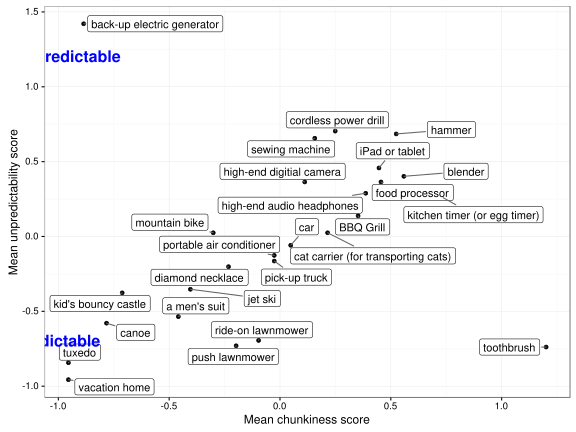
\includegraphics[width = \linewidth]{./plots/granularity_versus_predictability.pdf} 
\emph{Notes:} Scatter plot showing mean predictability versus chunkiness. 
\end{minipage} 
\end{figure} 

For each good, respondents were asked to rate the unpredictability of usage on a 1-5 scale (1 was highly predictable and 5 was highly unpredictable) as well as chunkiness (1 was one big chunk--- and 5 was low chunkiness---lots of little chunks).  
Figure~\ref{fig:granularity_v_predictability} plots the mean unpredictability score against the mean chunkiness score. 
We can see a strong relationship between chunkiness and predictability, with two notable outliers: the toothbrush and the generator. 
A toothbrush is used in small chunks (2 minutes according to the ADA) and its usage is highly predictable (after every meal, according to the ADA).
The back-up electric generator is the toothbrush's opposite---power can go out for days or even weeks during a disaster and this event is rarely predictable. 
These common-sense answers are not particularly illuminating but they do show subjects were paying attention and offering reasonable answers. 

If we examine goods near the origin (shaded green in the figure), we see goods highly amenable to rental, in that they have predictable usage that occurs in large chunks. 
Not surprisingly, these are often goods for which conventional rental markets already exist---formal wear (tuxedos), vacation homes, sporting equipment (canoes and jet skis for rent at lakes) and so on.
As we move a bit further, from the origin, we see goods that there is not much of a rental market (bikes, lawnmowers, jewlry) but would seem to have the attributes necessary to support such a market, assuming there are in fact enough non-owners to support such a market.  

\subsection{Chunkiness, predictability and ownership} 

We test whether the predictability and chunkiness measures are related to individual ownership. 
Table~\ref{tab:ownership_attr} shows that they are, in the expected direction:
\important{goods with unpredicatable usage that occurs in small chunks are substantially more likely to be owned.}
Furthermore, it is not the case that these two measures are simply capturing some single latent ``rentability'' measure, as both seem to have an independent effect on the probability of ownership. 


% Table created by stargazer v.5.0 by Marek Hlavac, Harvard University. E-mail: hlavac at fas.harvard.edu
% Date and time: Thu, Sep 25, 2014 - 09:53:36 PM
\begin{table}[!htbp] \centering 
  \caption{Good attributes and ownership---usage predictibility and granularity} 
  \label{tab:ownership_attr} 
\begin{tabular}{@{\extracolsep{5pt}}lccc} 
\\[-1.8ex]\hline 
\hline \\[-1.8ex] 
 & \multicolumn{3}{c}{\textit{Dependent variable:}} \\ 
\cline{2-4} 
\\[-1.8ex] & \multicolumn{3}{c}{Item is owned} \\ 
\\[-1.8ex] & (1) & (2) & (3)\\ 
\hline \\[-1.8ex] 
 Unpredictability index (UI) & 0.062$^{***}$ &  & 0.035 \\ 
  & (0.022) &  & (0.022) \\ 
  & & & \\ 
 UI x GI &  &  & $-$0.014 \\ 
  &  &  & (0.019) \\ 
  & & & \\ 
 Granularity index (GI) &  & 0.123$^{***}$ & 0.111$^{***}$ \\ 
  &  & (0.021) & (0.022) \\ 
  & & & \\ 
 Constant & 0.457$^{***}$ & 0.455$^{***}$ & 0.458$^{***}$ \\ 
  & (0.021) & (0.021) & (0.022) \\ 
  & & & \\ 
\hline \\[-1.8ex] 
Observations & 531 & 532 & 527 \\ 
R$^{2}$ & 0.015 & 0.061 & 0.065 \\ 
Adjusted R$^{2}$ & 0.013 & 0.059 & 0.060 \\ 
Residual Std. Error & 0.495 (df = 529) & 0.483 (df = 530) & 0.483 (df = 523) \\ 
F Statistic & 8.182$^{***}$ (df = 1; 529) & 34.342$^{***}$ (df = 1; 530) & 12.175$^{***}$ (df = 3; 523) \\ 
\hline 
\hline \\[-1.8ex] 
\end{tabular}
\\
{\footnotesize 
\begin{minipage}{0.90 \linewidth}
 \emph{Notes:} Here are some notes.
\end{minipage}
}
\end{table}
 

Column~(1) of Table~\ref{tab:ownership_attr} reports an estimate of 
\begin{align}
  \text{Own}_{ig} = \beta_0 + \beta_1 \textsc{UnpredictabilityScore}_{ig} + c_i + \epsilon_i
\end{align} 
where $\textsc{UnpredictabilityScore}_{ig}$ is the normalized predictability score for good $g$ by respondent $i$.
The coefficient on the unpredictability score is positive and highly significant, with a one standard deviation decrease in predictability increasing the probability of ownership by about 14 percentage points. 
In Column~(2) we instead use the chunkiness measure as the predictor and also find a positive and highly significant effect of about the same magnitude. 
In Column~(3) we interact the the chunkiness and predictability measures.
Each measure has a slightly smaller effect (though a formal hypothesis test would fail to reject a difference relative to the estimate when each measure appeared alone) and while the interaction term is negative, it is small and far from significant.

One concern with our approach might be that respondents prone to reporting high or low chunkiness and predictability scores might be idiosyncratically more or less likely to own the good.
In other words, the patterns from Columns~(1) through (3) reflect individual differences rather than general attributes about the good.
In Column~(4) we use the same specification as Column~(3) but include a good-specific effect.
With this effect, the coefficients on all regressors become close to zero, which supports the notion that the patterns in the previous regressions really are driven by the nature of the good. 

\subsection{Aggregate ownership and renting patterns at the level of the good}

This paper was motivated by the fact that P2P rental markets are \emph{begining} to flourish.
As such, asking respondents whether they have rented a particular good in a P2P rental market would likely yield uninteresting results, given how new they are.
However, the existing P2P rental markets seem to be focusing on sectors whether rental markets already existed, and so asking respondents if they have ever rented a good at all might be a reasonably proxy for whether they would eventually rent such a good in a P2P rental market. 
For each good, we asked whether the respondent's household (a) owned the good and (b) had ever rented the good.
As Figure~\ref{fig:scatter} will show, renting and owning are gross substitutes in data, when cars are excluded, as cars show a high level of both ownership and rental. 

\begin{figure}
\centering 
\caption{Fraction renting versus fraction owning \label{fig:scatter} }
\begin{minipage}{0.60 \linewidth}
\includegraphics[width = \linewidth]{./plots/scatter_rent_v_own.pdf} 
\end{minipage} 
\end{figure} 

In Figure~\ref{fig:scatter}, the fraction owning is plotted on the x-axis and the fraction renting on the y-axis.
Some notable goods are labeled---see Appendix~\ref{sec:additional_results} for the precise by-good fractions for every good.
The plot shows that there is generally a negative relationship between owning and renting, with the notable exception of cars.

Unsurprisingly, goods with nearly universal ownership show little renting with the notable exception of cars, which are both owned and rented at high rates.  
\important{There are a number of goods (not all labeled) that show medium ownership levels (e.g., around 50\%) and yet zero recorded instances of renting, which could indicate potential P2P rental market candidates.} 
Goods that are used during special occasions like weddings, celebrations and vacations show the highest rates of rental and lowest rates of ownership, e.g., tuxedos, vacation homes, jet ski, tuxedos, canoes, bouncy castles. 
There may also be some evidence of expensive tools useful for one-off jobs being rented, such as an electric generator and a pick-up truck. 


% Table created by stargazer v.5.0 by Marek Hlavac, Harvard University. E-mail: hlavac at fas.harvard.edu
% Date and time: Tue, Oct 07, 2014 - 02:28:57 PM
\begin{table}[!htbp] \centering 
  \caption{Fraction of respondents owning a good versus fraction having rented a good} 
  \label{tab:own_vs_rent} 
\begin{tabular}{@{\extracolsep{5pt}}lcc} 
\\[-1.8ex]\hline 
\hline \\[-1.8ex] 
 & \multicolumn{2}{c}{\textit{Dependent variable:}} \\ 
\cline{2-3} 
\\[-1.8ex] & \multicolumn{2}{c}{Rental Fraction} \\ 
 & All goods & Cars Excluded \\ 
\\[-1.8ex] & (1) & (2)\\ 
\hline \\[-1.8ex] 
 Ownership Fraction & $-$0.009 & $-$0.160$^{***}$ \\ 
  & (0.109) & (0.046) \\ 
  & & \\ 
 Constant & 0.081 & 0.115$^{***}$ \\ 
  & (0.059) & (0.024) \\ 
  & & \\ 
\hline \\[-1.8ex] 
Observations & 26 & 25 \\ 
R$^{2}$ & 0.0003 & 0.345 \\ 
Adjusted R$^{2}$ & $-$0.041 & 0.317 \\ 
Residual Std. Error & 0.176 (df = 24) & 0.071 (df = 23) \\ 
F Statistic & 0.006 (df = 1; 24) & 12.127$^{***}$ (df = 1; 23) \\ 
\hline 
\hline \\[-1.8ex] 
\end{tabular}
\\{\footnotesize \begin{minipage}{0.75 \linewidth} \emph{Notes:}
The unit of observation for the regressions in this table is the individual good.
The dependent variable is the graction of respondents reporting having rented that good, while the indendent variable is the fraction reporting owning that good. 
Column~(1) includes all goods surveyed, while Column~(2) excludes cars.
For the full list of goods and the survey langugage, see Appendix~\ref{sec:survey}. 
\starlanguage \end{minipage} }
\end{table}


To confirm the visual pattern of renting declining in ownership, Column~(1) of Table~\ref{tab:own_vs_rent} reports an estimate of 
\begin{align}
\textsc{FracRent}_g = \beta_0 + \beta_1 \textsc{FracOwn}_g + \epsilon,  
\end{align} 
where $\textsc{FracOwn}_g$ is the fraction of respondents claiming to own good $g$ and $\textsc{FracRent}_g$ is the faction claiming to have rented good $g$.
Column~(1) reports the estimated regression of this equation with cars, while in Column~(2), cars are excluded.
\important{If we exclude cars, there is a strong negative relationship between owning and renting, with a 10\% increase in the fraction owning reduces the fraction of households reporting renting by a little more than 1.5 percentage points. }

\section{Conclusion} 

One area where P2P rental markets could have a long-term effect is on the diversity of goods consumed. 
Consider that in some formulations of the consumer problem, consumers consume some positive amount of every good offered.
This is obviously a large departure from empirical reality if we draw fine-grained distinctions between ``goods.'' 
For example, Amazon.com currently lists 6,238 results for ``blender'' in the Home \& Kitchen category: 
presumably most households own far fewer than this, with most owning one or none.\footnote{As of October 8th, 2014.}
The reason for this pattern in the language of this model is clear: 
a consumer's $\alpha$ for Blender 2 \emph{conditional} upon owning Blender 1 is quite low and so another blender is not purchased.
However, if a rental market existed for both blender types, consumers could act upon their taste for diversity without owning a dozen blenders. 
Even if the blender example seems implausible, we should consider that very few consumers try to rent the car they normally drive or vacation in their hometown: presumably they diversify consumption in these cases precisely because they can. 

One long-term reaction to the rising of P2P rental markets is that firms might change the goods that they offer. 
As P2P rental markets become commonplace, manufacturers will begin designing products more attractive for this additional purpose. 
For example, locks on cars and houses that allow remote entry will be more appealing. 
The emerging Internet-of-Things will make it easier to identify goods that are not being used at a moment in time and perhaps facilitate trade automatically.
If autonomous vehicles and drones become commonplace, even the seemingly unavoidable transaction costs associated with moving goods to where they are needed might be substantiall diminished.\footnote{Thanks to Jonathan Hall for making this point.}
Similarly, technologies that make it easier to monitor usage (GPS, embedded sensors, streaming video of how they are being used and so on) should make contracting easier and reduce some of the informational asymmetries that contribute to transaction costs. 
As more of economic and social life are computer-mediated, platforms will use this information to verify the identify and reputation of buyers and sellers, further mitigating moral hazard and adverse selection.  

One area not considered by this paper how many of these P2P rental markets also have an inherent labor input. 
For normal goods, we might expect owners to have higher opportunity costs of time, which would tend to reduce the supply given their higher labor costs.
We might also see more platforms where the labor input is provided by a firm (or even the P2P rental market platform itself) but the capital is still provided by the good owner;
this would be similar to the property manager role common in real estate.

Our model makes several predictions that are---or should become---testable over time, as P2P rental markets grow.
Some obvious candidates include examining whether the emergence of P2P rental markets increase access by non-owners, changes the ownership decision and affects rental rates.
Given the substantial legal and regulatory obstacles many sharing economy companies face---including being banned in some places at certain periods of time---might make credible quasi-experimental designs feasible. 

% \cite{ikkala2014defining}

\bibliographystyle{aer}
\bibliography{sharing.bib}

\newpage 

\appendix 

\section{Survey Questions \label{sec:survey}} 

The actual goods were: 

\begin{itemize} 
\item BBQ Grill
\item toothbrush
\item a men's suit
\item blender
\item canoe
\item car
\item cordless power drill
\item hammer
\item diamond necklace
\item food processor
\item hammer
\item cat carrier (for transporting cats)
\item high-end audio headphones
\item high-end digitial [sic] camera
\item iPad or tablet
\item jet ski
\item kid's boucy [sic] castle
\item kitchen timer (or egg timer)
\item mountain bike
\item pick-up truck
\item push lawnmower
\item ride-on lawnmower
\item tuxedo
\item vacation home
\item back-up electric generator
\item portable air conditioner
\item sewing machine
\end{itemize} 

\begin{itemize} 

\item Does your household own a {\bf good}?
\begin{itemize}
\item Yes
\item No
\end{itemize} 

\item Have you ever lent your {\bf good} to someone else?
\begin{itemize}
\item Yes
\item No
\item NA - we do not own one.
\end{itemize} 

\item Have you ever borrowed a {\bf good} from someone else?
\begin{itemize}
\item Yes
\item No
\item NA - we own one.
\end{itemize} 

\item Have you ever rented a {\bf good}?
\begin{itemize}
\item Yes
\item No
\item NA - we own one.
\end{itemize} 

\item Regardless of whether your household owns a {\bf good}, if you did own one, how much do you estimate it would be used by members of your household on average?

\begin{itemize} 
\item We would not use this at all
\item 1 minute a week (about 1 hour a year) 
\item 5 minutes a week (about 4 hours a year)
\item 1/2 an hour a week
\item 1 hour a week
\item 1/2 an hour a day
\item 1 hour a day
\item 2 hours a day
\item 4 hours a day
\item 8 hours a day
\item 16 hours a day
\item 24 hours a day (I would continuously be using this good)
\end{itemize} 

\item Regardless of whether you actually own a {\bf good}, how do you imagine it would be used if it was owned by your household (on a scale of 1 to 5): 
\begin{itemize} 
\item 1 - Used in one big block of time
\item 2  
\item 3 - Used in a mixture of large and small blocks of time
\item 4 
\item 5 - Used in many small blocks of time
\end{itemize} 

\item Regardless of whether you actually own a {\bf good}, how predictable would your usage of it be if you did own it: 
\begin{itemize}
\item 1 - Very predictable---I can plan usage many weeks in advance
\item 2  
\item 3 - Somewhat predictable 
\item 4 
\item 5 - Very unpredictable---I would never know exactly when I would need to use it until right beforehand. 
\end{itemize} 

\item If you do not own a {\bf good}, what is the primary reason?
\begin{itemize} 
\item NA - we own one.
\item We wouldn't use it enough to justify the purchase price
\item We would use it, but we simply do not have the money.
\item I don't have the space for this item
\end{itemize} 

\item What is your total household income? 
\begin{itemize} 
\item Less than \$10,000
\item  \$10,000-\$19,999
\item  \$20,000-\$29,999
\item  \$30,000-\$39,999
\item  \$40,000-\$49,999
\item  \$50,000-\$59,999
\item  \$60,000-\$69,999
\item  \$70,000-\$79,999
\item  \$80,000-\$89,999
\item  \$90,000-\$99,999
\item  \$100,000-\$149,000
\item  More than \$150,000
\end{itemize} 

\end{itemize}

\section{Additional empirical results} \label{sec:additional_results}

Figure~\ref{fig:frac_owning} shows the fraction of respondents reporting owning various goods, as well as 95\% confidence intervals for that point estimate computing using the Wilson method for a binary proportion.    
There are few surprises: nearly everyone owns a toothbrush, a hammer and a blender; no one reported owning a jet ski and only one respondent reported owning a vacation home.
Figure~\ref{fig:frac_renting} shows the fraction of respondents reporting having rented the various goods. 
\important{Generally, ownership and renting appear to be gross substitutes, with the notable exception of cars, presumably because people rent cars when traveling.}

\begin{figure}
\centering 
\caption{Fraction of respondents owning various goods \label{fig:frac_owning} }
\begin{minipage}{0.90 \linewidth}
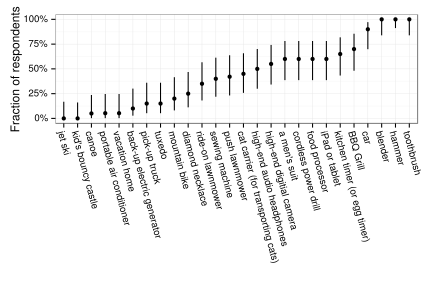
\includegraphics[width = \linewidth]{./plots/ownership_fractions.pdf} 
\end{minipage} 
\end{figure} 

\begin{figure}
\centering 
\caption{Fraction of respondents reporting having rented various goods \label{fig:frac_renting}}
\begin{minipage}{0.90 \linewidth}
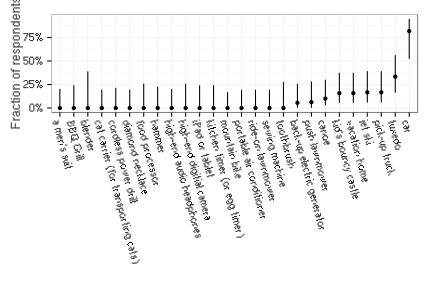
\includegraphics[width = \linewidth]{./plots/rental_fractions.pdf} 
\end{minipage} 
\end{figure} 

The mean unpredictability scores by good seem sensible: 
Figure~\ref{fig:predict_index} shows the mean unpredictability index per good. 
The most predictable goods are either those associated with planned recreation (e.g., vacation home, canoe, jet ski, tuxedo) or predictable chores (e.g., toothbrush, the two kinds of lawnmowers). 
The most unpredictable goods are associated with either food preparation (e.g., blender, food processor) or repairs (e.g., hammer, sewing machine, cordless power drill). 
Back-up electric generator is a clear (and unsurprising) outlier---you are in a sense always ``surprised'' when you need to use it. 


\begin{figure}
\centering 
\caption{Mean unpredictability index by good \label{fig:predict_index} }
\begin{minipage}{0.90 \linewidth}
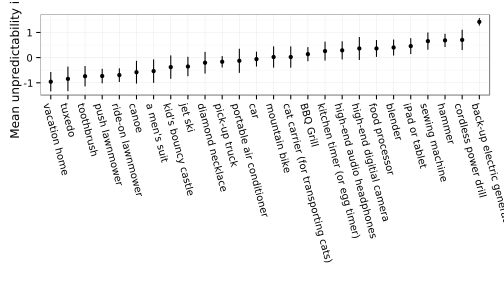
\includegraphics[width = \linewidth]{./plots/predictability.pdf} 
\end{minipage} 
\end{figure} 

Figure~\ref{fig:granularity} shows the mean chunkiness index per good. 
There appears to be some similarity in high predictable usage, but some goods used in small chunks of time also appear to have highly predictable usage---namely the toothbrush. 
To make this relationship explicit, in Figure~\ref{fig:granularity_v_predictability} the chunkiness and predictability indices are plotted against each other. 
\important{With the exception of two goods---the toothbrush and back-up generator---predictability and chunkiness are strongly positively correlated.}

\begin{figure}
\centering 
\caption{Mean chunkiness index by good \label{fig:granularity}}
\begin{minipage}{0.90 \linewidth}
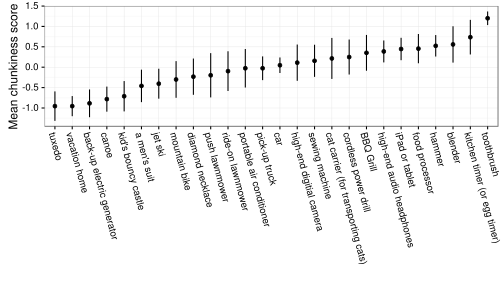
\includegraphics[width = \linewidth]{./plots/granularity.pdf} 
\end{minipage} 
\end{figure} 

\end{document} 

\section{New New Stochastic Model}

A would-be-user of some good learns their valuation from using that good that period.
That value is $v \sim U[0,1]$.
The owner always has the outside option $\underline{u}$ of using some other good. 
If $v > \underline{u}$, the use the good, otherwise they do not.
The realized utility from owning the good is thus:
\begin{align}
  \int_{\underline{u}}^1 v dv = \frac{1}{2} - \frac{\underline{u}^2}{2}
\end{align} 
This determines their purchase decision---if the pro-rated purchase price is less than the utility, then they buy, otherwise they do not.
Assume that a fraction of consumers $\theta$ own the good and $(1-\theta)$ do not. 

The owners of the good can rent to the non-owners at a market-clearing rental rate of $r$, after paying a transaction cost of $c$. 
We first note that if $c > r$, then no owner chooses to rent out the good and there would be no supply to the market.
For $r - c > 0$, the owner would be willing to rent some of the time.
For $r - c < \underline{u}$, the owner would simply rent out during periods when they would not have used the good anyway.
This occurs $\underline{u}$ of the time and so the market supply would simply be $\underline{u}\theta$.
For a sufficiently high rental rate, the owner would also economize of their usage, renting out during some relatively low-value periods when they otherwise would have consumed.
For $r - c > \underline{u}$, market supply is $\theta (r - c)$.
The supply curve (plotted in Figure~\ref{fig:supply}) is 
\begin{align}
S(r) =  \left\{
     \begin{array}{ll}
       0                       & : 0 > r - c  \\
       \theta \underline{u}    & : 0 < r - c < \underline{u} \\ 
       \theta (r - c)          & : \underline{u} < r - c   
     \end{array}
   \right. 
\end{align} 

\begin{figure}
\centering 
\caption{Short-run P2P rental market supply curve}
\label{fig:supply} 
\begin{minipage}{0.50 \linewidth}
  \includegraphics[width = \linewidth]{./figures/supply_curve.png} \\
  \begin{footnotesize}
  \emph{Notes}: Here is a supply curve. 
  \end{footnotesize}
\end{minipage}
\end{figure} 

On the demand side, a non-owner is willing to rent if $v - r > \underline{u}^R$, where $\underline{u}^R$ is the outside option of non-owners.
The demand curve is thus
\begin{align} 
D(r) =  \left\{
\begin{array}{ll}
      (1 - \theta) ( 1- \underline{u}^R)   & : r < \underline{u}^R \\
      (1 - \theta) (1 - r)            & : r > \underline{u}^R 
     \end{array}
   \right. 
\end{align} 

\begin{figure}
\centering 
\caption{Short-run P2P rental market demand curve}
\label{fig:demand} 
\begin{minipage}{0.50 \linewidth}
  \includegraphics[width = \linewidth]{./figures/demand_curve.png} \\
  \begin{footnotesize}
  \emph{Notes}: Here is a demand curve. 
  \end{footnotesize}
\end{minipage}
\end{figure} 

\subsection{Equilibrium}
There are several possibile equilibria.
TK - NOTE: I have not worked out the conditions under which these different equilibrium arise.
Not all might be possible, especially if we assume (reasonably) that $\underline{u} < \underline{u}^R$. 

\paragraph{No trade equilibrium} 
If $c$ is sufficiently high, then the good is not transacted at all.
This would occur if $c > 1$, as $v = 1$ is the highest possible valuation a non-owner can have for the good.

\paragraph{``Owners consume the same'' equilibrium}
There is an equilibrium where the vertical portion of the supply curve---where only unused capacity is sold---intersects the sloping portion of the demand curve, or $\theta \underline{u} = (1 - \theta)(1 - r)$, 
which gives a market-clearing rental rate of
\begin{align}
  r = 1 - \underline{u} \left( \frac{\theta}{1 - \theta} \right).
\end{align} 
As we would expect, as the relative number of owners increases, rental rates fall.
The higher the value of $\underline{u}$, the greater the fraction of time owners would not have used the good anyway, and hence the greater supply and lower rental rates.

\paragraph{``Owners and non-owners economize on usage'' equilibrium} 
There is an equilibrium where sloping portions of the two curves intersect, giving a market-clearing rental rate of
\begin{align}
  r = 1 - \theta(1 - c).
\end{align} 
As transaction costs rise, the rental rate increases.
As expected, more owners lowers the rental rate, as this increases supply on the market. 

\paragraph{``Owners economize but non-owners do not'' equilibrium} 
In this equilibrium, the sloping portion of the supply curve intersects the vertical portion of the demand curve, giving an equilibrium rental rate of 
\begin{align}
  r = c + \left( \frac{1 - \theta}{\theta } \right) (1 - \underline{u}^R)
\end{align} 

When $\underline{u}^R$ is goes up, there is less demand and so rental rates fall.
Rental rates are increasing in the transaction costs.
The greater the relative number of non-owners, the higher the rental rate.


\section{New stochastic model} 
In each period, a consumer would get some value from using a good with probability $q$. 
If they want to use the good, they would get a value $v \sim U(0, 1]$. 
The outside option of not using the good is $0$ and so for all realizations of $v$, they would use the good. 
A user will thus own the good if $q \mathbb{E}[v] > p$, where $p$ is the purchase price amortized over the lifetime of the good, which we assume is independent of usage. 


\subsection{Short-run P2P rental market equilibrium} 

Assume that consumers differ in their expected usage, with $q_H > q_L$. 
The fraction of consumers with $q_H$ is $\theta$. 
Assume the purchase price and value distribution is such that the high-types own and the low-types do not. 
High-types can rent the good out for $r$, the market rental rate, but it costs $c$ to bring the good to market.
If $r > c$, then the owner of the good will rent out on all of the non-use days, which is $1-q_H$ of the time. 
They will also rent out on their planned use days whenever the expected value from usage is below the rental rate, less the transactions costs, or $v < r - c$. 
This occurs with probability $r - c$. 
For the low-types, when they have a usage day (which happens with probability $q_L$), they wish to rent whenever $v > r$. 

The supply curve is 
\begin{align}
S(r) =  \left\{
     \begin{array}{ll}
       0                       & : r < c \\
       \theta \left ( (1 - q_h) + (r - c)q_H \right)  & : r > c
     \end{array}
   \right. 
\end{align} 
while the demand curve is 
\begin{align}
D(r) = (1 - \theta) q_L (1 - r)  
\end{align} 


\subsection{Short-run surplus in the P2P rental market} 
\subsection{Long-run P2P rental market equilibrium} 


We can see that the high-types, as the bearers of the transaction costs are more likely to consume than low-types. 

Sharing causes owners to economize of on low-value usage, transferring it to non-owners with a higher valuation. 


The slope of the supply curve if $\theta q_H$. 
The fixed component $c$ shifts the curve in and out.  


\begin{align} 
(1-\theta) q_L (1 - F(r))  = \theta \left ( (1-q_h) + q_h F(r - c) \right)
\end{align} 

\begin{align} 
(1-\theta) q_L (1 - r)  = \theta \left ( (1-q_h) + q_h (r - c \right)
\end{align} 

What does the long-run market equilibrium look like? 
No one would want to switch their ownership decision. 

They get rental income on the $v < r - c$
The utility from owning for a high-type: 
\begin{align}
U^{OWN}_H = (1 - q_H) r + q_h \left( r \mbox{Pr}\{v < r - c\} + \mbox{Pr}\{v > r - c\} \mathbb{E}[v > r - c] \right) - p
\end{align} 

A high-type only rents if $v > r$. 
\begin{align}
U^{RENT}_H = q_h \mathbf{E}[v - r | v > r]. 
\end{align} 


For the first case, high-types have to be indifferent between owning and renting.
With bringing-to-market costs, high-type owners have more consumption than high-type owners, as owners face a marginal cost of $r-\gamma$, while non-owners face the full $r$.
As high-type renters are renting from high-type owners, for the renters to stay indifferent, they have to get passed a transfer equal to the cost of foregone consumption.

High-type owners get $\alpha_H^2 - (r-\gamma)^2/4$ in consumption utility, while renters get $\alpha_H^2 - r^2/4$.

We know that $r_{LR} - \gamma \le p$, otherwise an individual could buy the good, rent it all out and make a profit. 

Is $r_{LR} = p + \gamma$?
If it is, high-type owner consumes $\alpha_H - r/2 = \alpha_H - (p + \gamma)/2$, while a high-type consumes $\alpha_H - p/2$. 
The total utility for high-types owning would then be $\alpha_H^2 - p^2/4 + (1 - (\alpha_H - p/2))p - p$.

The total utility for high-types renting would then be $\alpha_H^2 - (p - \gamma)^2/4 - (\alpha_H - (p + \gamma)/2)(p + \gamma)$.

$\Delta U = \frac{1}{4}(2r - \gamma)\gamma$.
Owners bear a cost equal to $p + (1 - (\alpha - (r - \gamma)/2))\gamma$. 

%% $D(p) = \theta \alpha_H + (1 - \theta) \alpha_L - p/2$, and so $\bar{p}_{1} = 2[\theta \alpha_H + (1-\theta)\alpha_L]$. 
%% \important{Since $\alpha_H > \alpha_H^2$ and $\alpha_L > 0$, $\bar{p}_1 > \bar{p}_0$: the existence of a P2P rental market can support a higher product market price.} 
%% Figure~\ref{fig:demand} illustrates the new product market demand curve, with the pre-P2P rental market curve indicated as $D_0$ and the post-P2P rental market by $D_1$. 
%% % http://tex.stackexchange.com/questions/76418/plot-non-continuous-function-with-tikz
%% \begin{figure}
%% \caption{Product market demand pre-P2P rental market and post-P2P rental market (long-run)}
%% \label{fig:demand} 
%% \centering
%% % \begin{tikzpicture}[scale=5]
%% % \draw (1,0) node[below]{$Q$} -- (0,0) --(0,1) node[left]{$p$};
%% % \draw[ultra thick] (0,1) to (0, \alphaH^2); 
%% % \draw (0,\alphaH^2) circle (1pt)
%% % \end{tikzpicture}
%% \includegraphics[scale = 1]{./diagrams/p2plr_demand.pdf}
%% \end{figure} 


%% Figure~\ref{fig:demand} shows this and it shows that with the P2P rental market in long-run equilibrium, demand can be non-zero above this point.  
%Intuitively, if a would-be owner can earn rental income from their unused capacity, it seems likely that a higher product market price is supportable. 

%% In this high-price range, the $D_1$ curve is kinked at $p = 2\alpha_L$. 
%% \important{The reason for this kink is that if $2\alpha_L < p$, the low-types do not use the good in the long-run P2P equilibrium.} 
%% The reason is simple: if $p > 2\alpha_L$, usage of the good offers negative utility from any amount of usage and so the low-types use none. 
